\documentclass[a4paper,10pt]{article}
\usepackage{luatexja}
\usepackage{luatexja-fontspec}
\usepackage{geometry}
\usepackage{multicol}
\usepackage{titlesec}
\usepackage{setspace}
\usepackage{graphicx}
\usepackage{caption}
\usepackage{indentfirst}
\usepackage{float} % 図の位置を制御するために追加
\usepackage{listings}
\usepackage{xcolor}

\geometry{margin=20mm}
\setstretch{1.2}
\parindent=1em

% ===== 日本語フォント設定 =====
% HaranoAjiMincho がシステムに入っている必要あり
\setmainjfont{HaranoAjiMincho} % メイン日本語フォント
\setsansjfont{HaranoAjiGothic} % サンセリフ(任意)
\setmonojfont{HaranoAjiMincho} % 等幅も同じに設定(好みに応じて変更)

% 図のキャプションの表記を「図1」のように日本語化
\renewcommand{\figurename}{図}
\captionsetup[figure]{labelformat=default,labelsep=period}

\renewcommand{\tablename}{表}
\captionsetup[table]{labelformat=default,labelsep=period}

\geometry{margin=25mm}
\setstretch{1.2}
\parindent=1em

\titleformat{\section}{\large\bfseries}{\thesection.}{1em}{}

\definecolor{keywordcolor}{rgb}{0.26, 0.38, 0.68}
\definecolor{commentcolor}{rgb}{0.3, 0.6, 0.3}
\definecolor{stringcolor}{rgb}{0.7, 0.2, 0.2}

\lstdefinelanguage{SystemVerilog}{
  morekeywords={module,endmodule,input,output,logic,always_ff,if,else,begin,end,posedge,negedge},
  sensitive=true,
  morecomment=[l]{//},
  morecomment=[s]{/*}{*/},
  morestring=[b]",
}

\lstset{
  language=SystemVerilog,
  basicstyle=\ttfamily\small,
  keywordstyle=\color{keywordcolor}\bfseries,
  commentstyle=\color{commentcolor}\itshape,
  stringstyle=\color{stringcolor},
  numbers=left,
  numberstyle=\tiny,
  stepnumber=1,
  numbersep=5pt,
  frame=single,
  tabsize=2,
  showstringspaces=false,
  breaklines=true,
  breakatwhitespace=true
}

\title{SystemVerilog Code with Listings}

\begin{document}

% タイトルブロック
\begin{center}
\noindent
{\LARGE 第3回輪講資料} \\
{\large 4321 野秋 琳太郎} \\
2025年 10月 02日
\end{center}

\begin{flushright}
指導教員 宮田 尚起
\end{flushright}

% 二段組開始
\begin{multicols}{2}[\raggedcolumns]
\section{はじめに}
LEDで光通信をして,「糸なし糸電話」をした.
ほかの近況報告としては,「岩波講座 現代の物理学〈2〉電磁力学」を半分(相対論の最初らへん)ぐらいまで読んだ.
きっと編入試験やら来年の研究やらで役にたってくれるであろう.

\section{やったこと}
\subsection{通信のプロトコルの整理}
前回,本橋の輪講資料にある通り,オーディオ信号を分解能8bitでデジタル信号に変換し,シリアル通信でデータを送る.
このシリアル通信は基本的にUARTの規格に沿ったものであるが,少々手が加えてある.
図\ref{fig:uart_protocol},\ref{fig:protocol}はそれぞれ,本来のUARTと「糸なし糸電話」用に手を加えた通信の波形である.
図\ref{fig:uart_protocol}で周期的に垂れ流され,ダミーbitがストップbitの役割をすることで,通常のUART受信回路を使用することができる.

今回使用する通信は途中で途絶えることが多い.
図\ref{fig:saikai_protocol}のようにデータを送っている途中で通信が開始した(再開した)場合を考える.
このとき,送信側と受信側で現れる波形は同一であるが,その意味は異なる.
まず,データが1から0になったタイミングで,受信回路はそれをスタートbitとして誤認する.
そして1bitぶんの時間を開けて,そこから8bitの信号をデータbitとしてゴミのデータを内部に取り込む.
ここで7bitぶんのダミーがあるので,次のスタートbitが来る前にデータの受信を完了する.
するとダミーbit(1)のあとのスタートbit(0)を,確実にスタートbitとして認識できる.
これにより,2周期目以降の通信では確実に正しいデータを得られるようになる.

\begin{figure}[H]
    \centering
    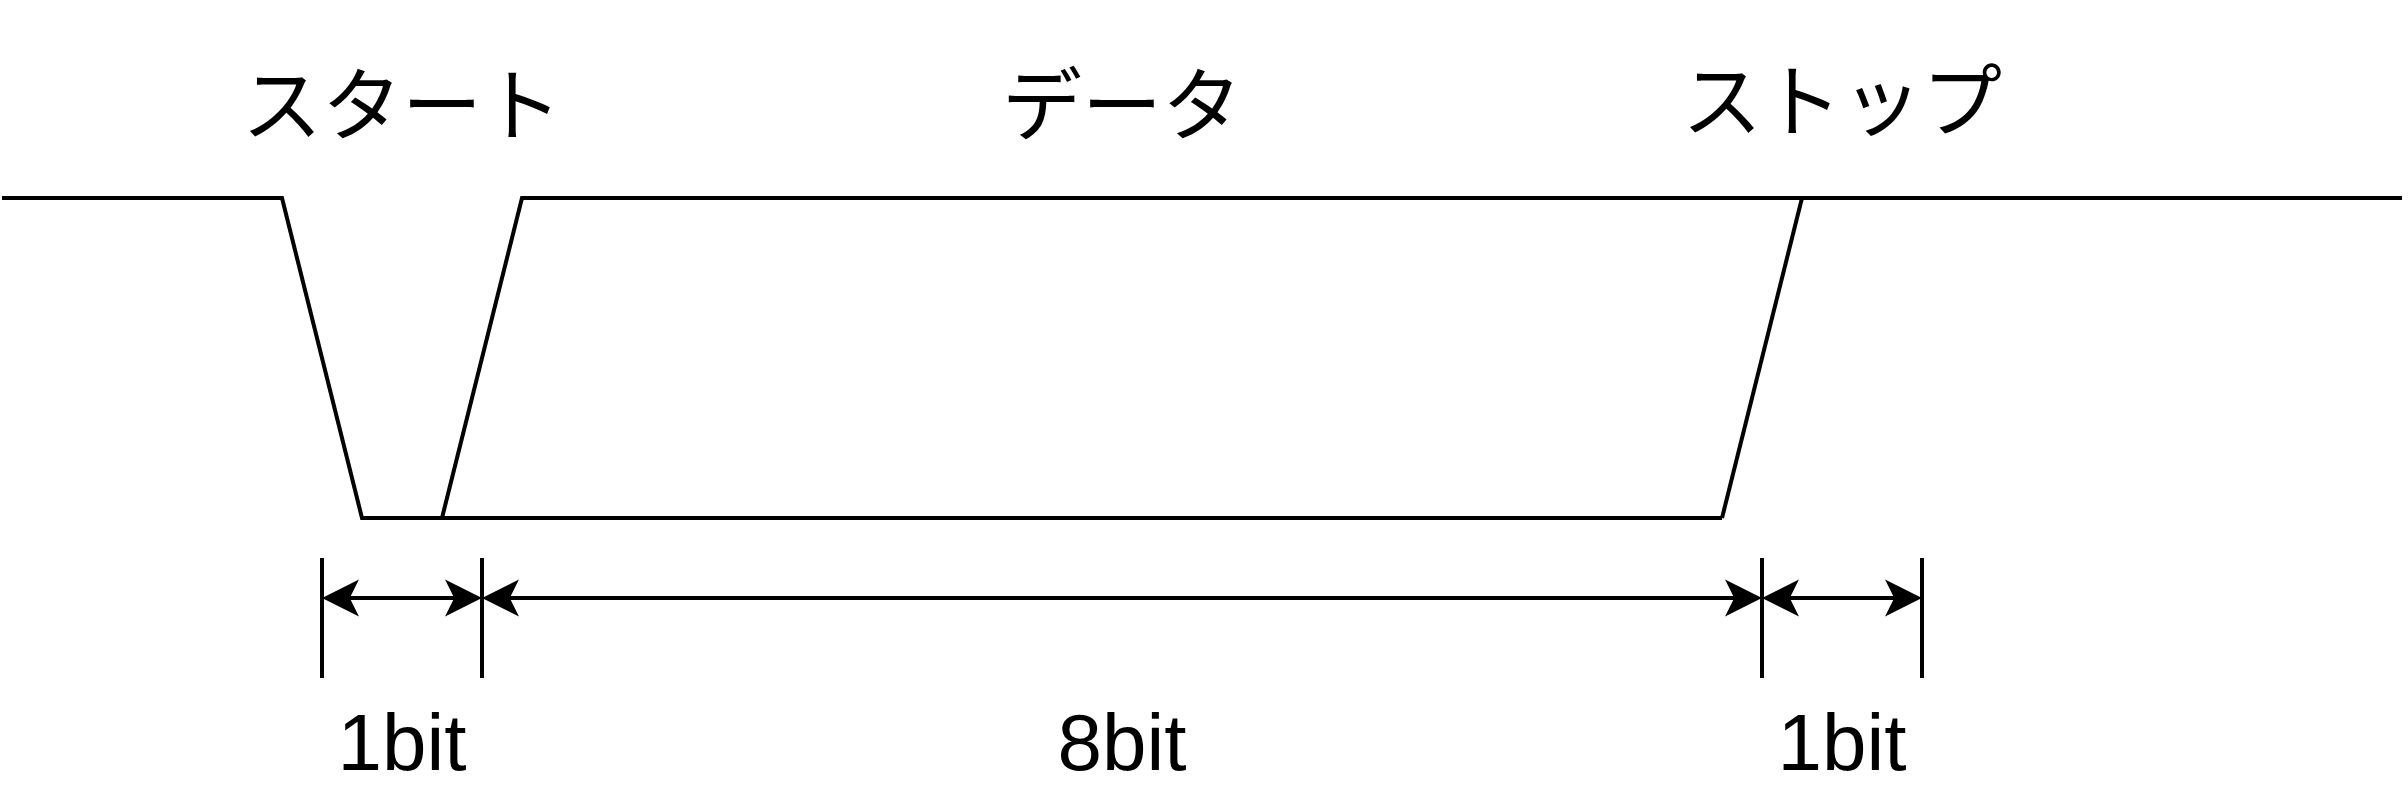
\includegraphics[width=0.9\linewidth]{figure/uart_protocol.png} 
    \caption{UART通信の波形} 
    \label{fig:uart_protocol}
\end{figure}
  
\begin{figure}[H]
    \centering
    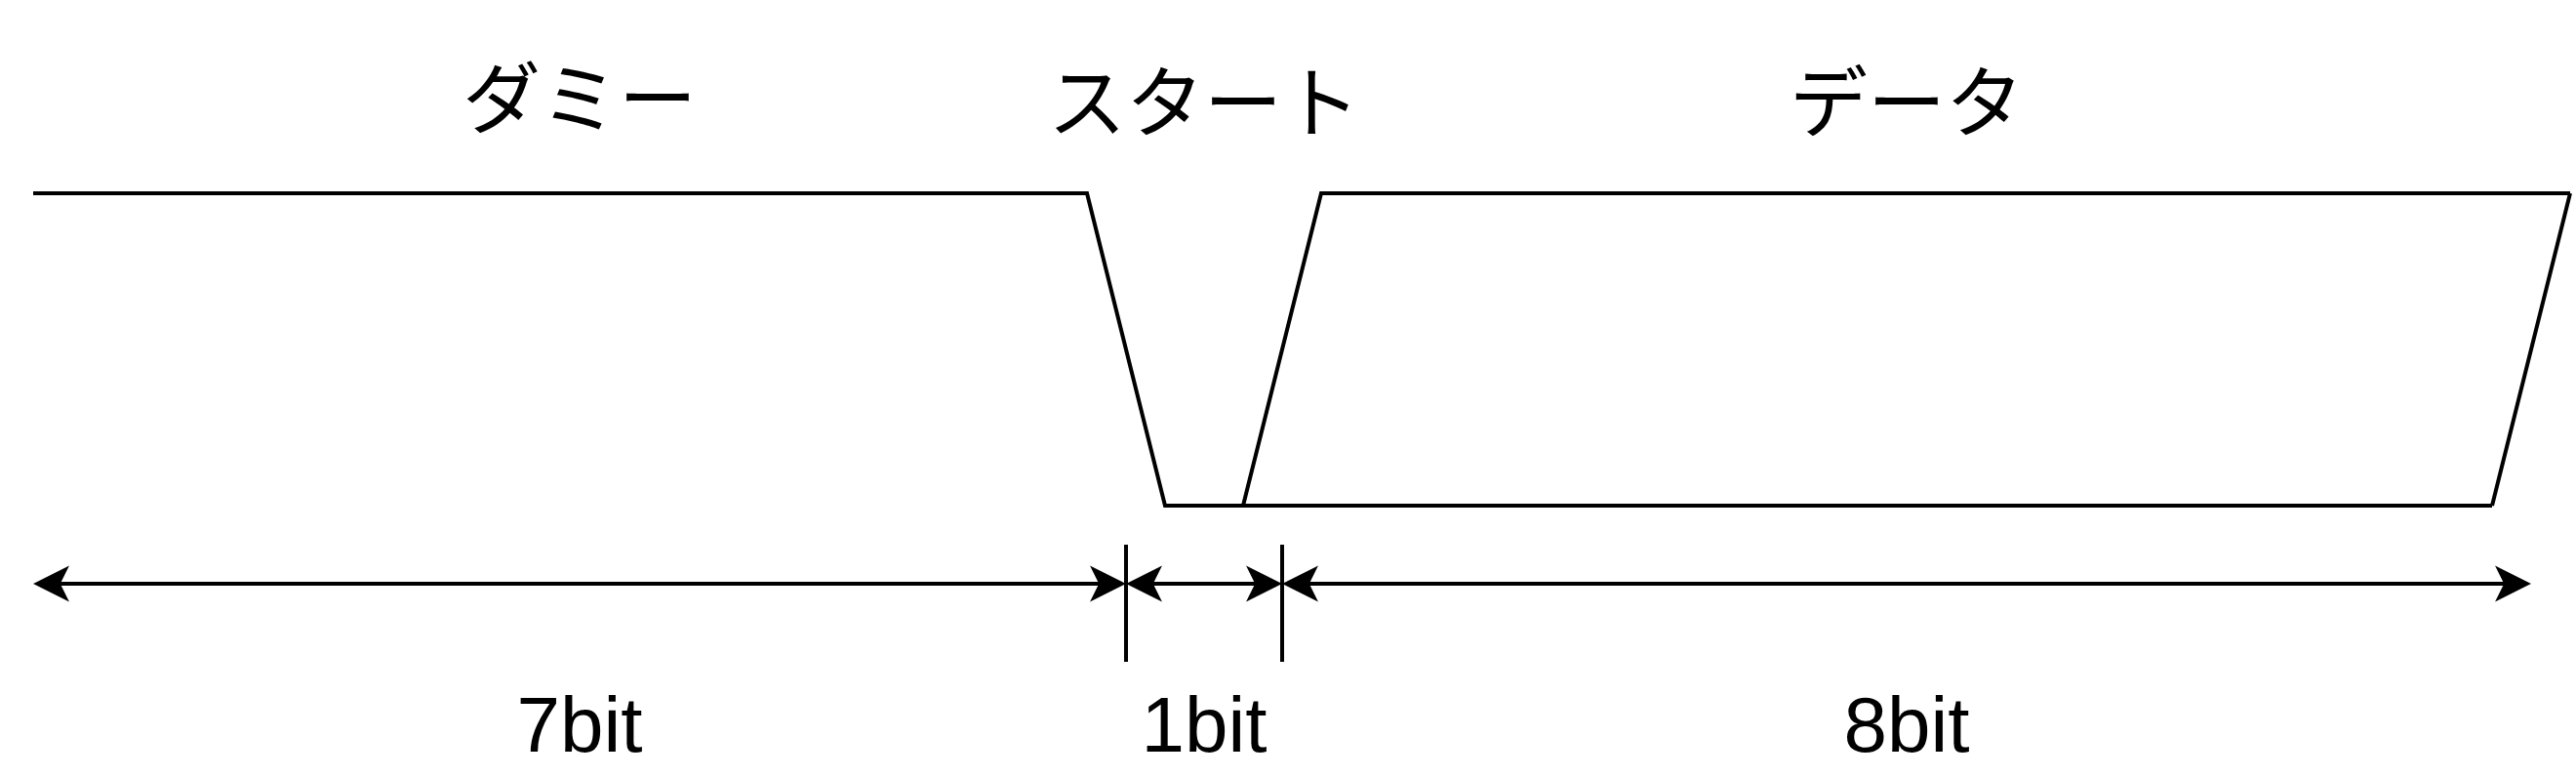
\includegraphics[width=0.9\linewidth]{figure/protocol.png} 
    \caption{使用する通信の波形} 
    \label{fig:protocol}
  \end{figure}

\begin{figure}[H]
    \centering
    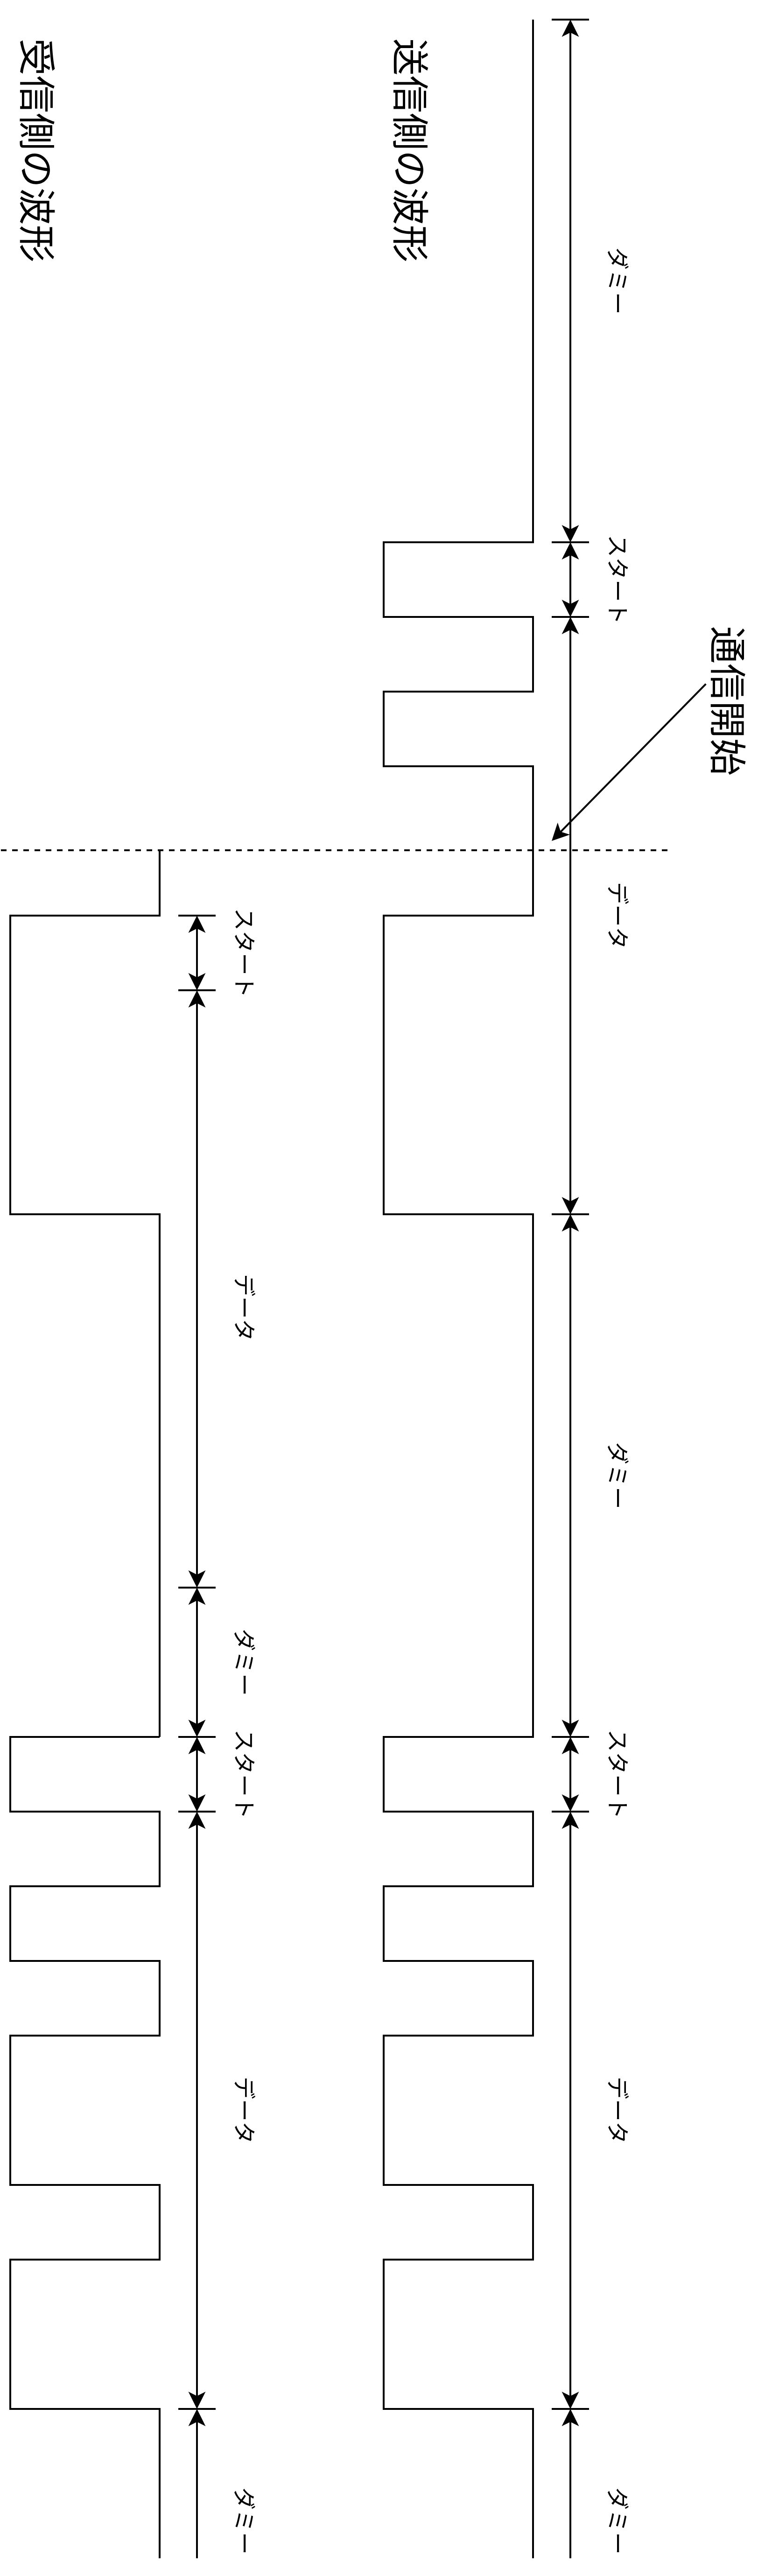
\includegraphics[width=0.6\linewidth]{figure/saikai_protocol.png} 
    \caption{データの途中で通信が開始した場合} 
    \label{fig:saikai_protocol}
\end{figure}

\subsection{回路図を描く}
糸なし糸電話のブロック図を図\ref{fig:block_diagram}に示す.
各ブロックの回路を以下で説明する.

\begin{figure}[H]
    \centering
    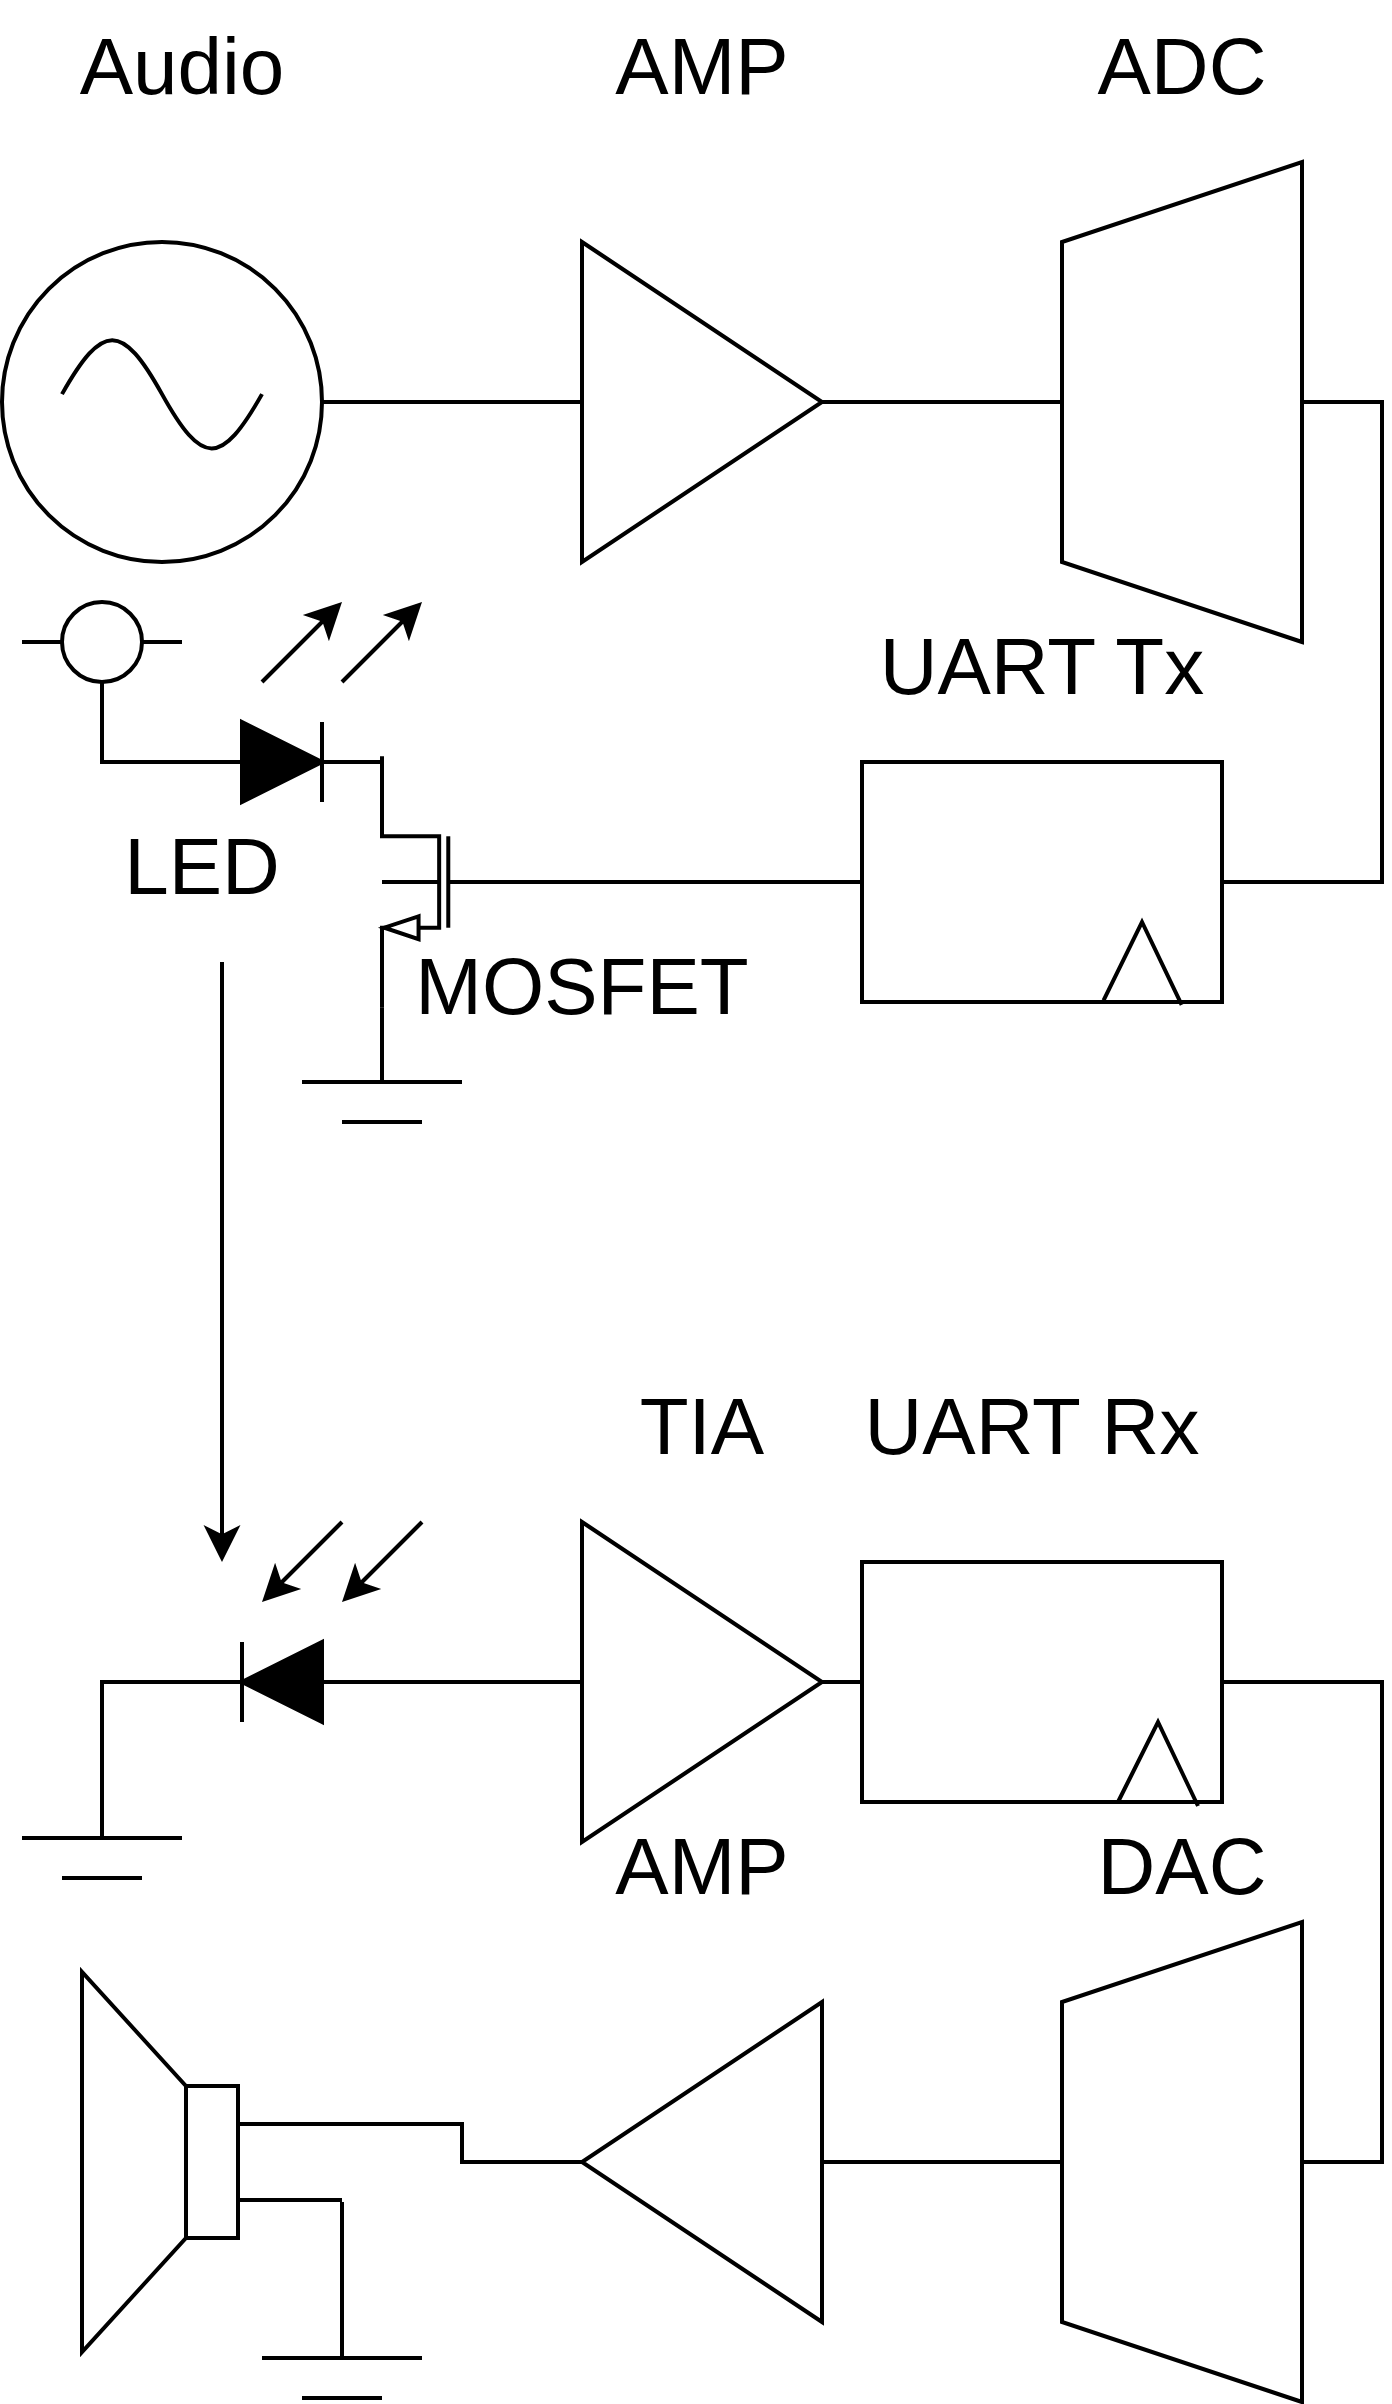
\includegraphics[width=0.8\linewidth]{figure/block_diagram.png} 
    \caption{糸なし糸電話のブロック図} 
    \label{fig:block_diagram}
\end{figure}

\subsubsection{入力側アンプ}
入力側アンプは図\ref{fig:in_amp}のように設計した.
このアンプは二段階になっていて,
  DCカット→バイアス→増幅→DCカット→バイアス→増幅
という構成になっている.
入力電圧の振幅は,パソコンなどのイヤホンジャックで数百mV,マイクの出力で数mVである.
そのため,アンプの増幅率は数十倍から数百倍のものが必要になる.
アンプを2段階にするとその調整が容易になる.

電源電圧に5V以外を用意するのは面倒なので,電源電圧5Vの単電源でレールtoレールに動作するOPアンプ,$MCP602$を使用した.
数mVオーダーで振れるオーディオ信号をOPアンプの動作点まで引き上げたいので,バイアス回路にかけてからOPアンプに入力するようにしている.

\begin{figure}[H]
    \centering
    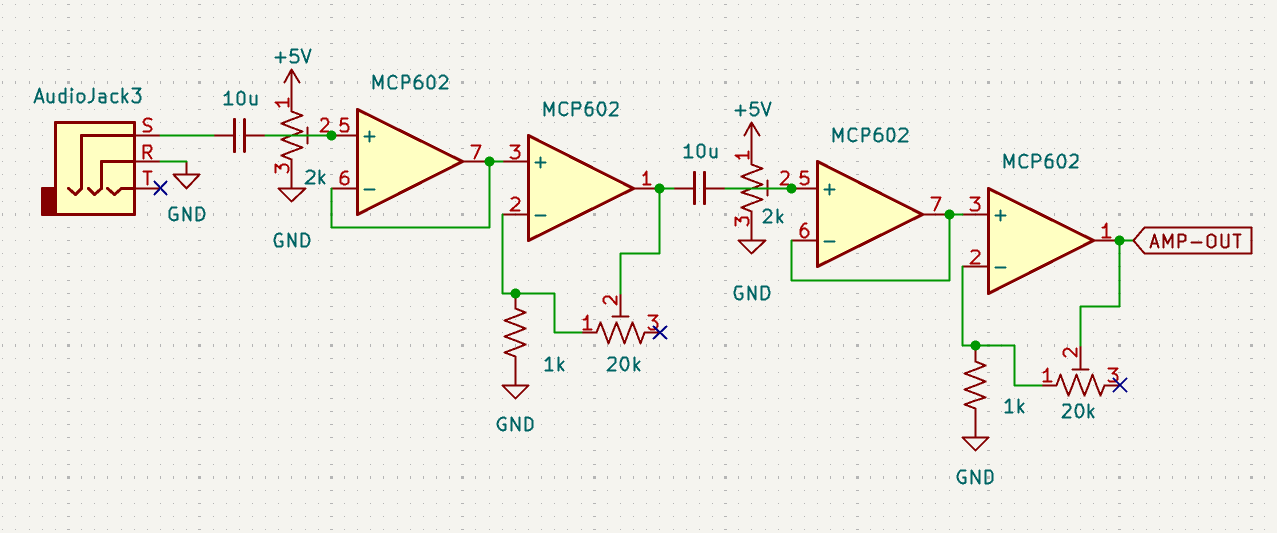
\includegraphics[width=1.5\linewidth,angle=270]{figure/in_amp.png} 
    \caption{入力側のアンプの回路} 
    \label{fig:in_amp}
\end{figure}

\subsubsection{ADコンバータ}
ADコンバータは図\ref{fig:adc}のように設計した.
使用したICは$\mu PD6950$である.
これは映像信号用のADコンバータで,14MHzで8bitの変換が可能である.

$ADC\_CK$はUARTのタイミング用の信号の分周元で,4.9152MHzが入力されている.
また,$RT$はADコンバータの基準電圧で3.5Vに調整して入力される.

\begin{figure}[H]
    \centering
    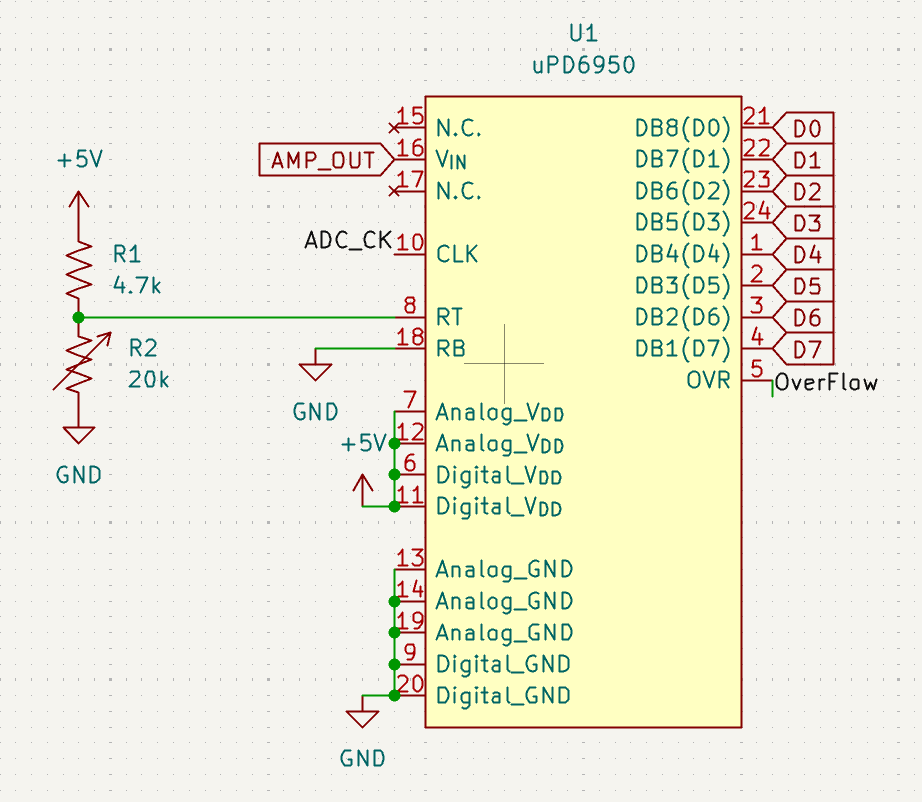
\includegraphics[width=0.9\linewidth]{figure/adc.png} 
    \caption{ADコンバータ} 
    \label{fig:adc}
\end{figure}

\subsubsection{UARTの出力}
UART出力回路は, 図\ref{fig:uart_tx}に示すように設計した.  
この回路の中心的な役割を担っているのは, 74LS165である.
74LS165の内部回路を図\ref{fig:74165}に示す.
74LS165は8bit幅のシフトレジスタであり, 本研究ではこれを2つ直列に接続することで, ダミーbitやスタートbit, そして実際のデータbitを含めた合計16bit分のデータをシフトできるようにしている.  
この構成により, UARTで必要とされるbit列を一定のリズムで送り出すことが可能となる.  

さらに, ダイオードロジックからの出力である$SHIFT\_LOAD$信号は, 16bit分のシフトが完了したタイミングでアサートされ,この瞬間に新しいデータをレジスタにロードする仕組みとなっている.  
ダミーbitやスタートbitを含め, あらかじめ決め打ちされたbit列を毎周期確実にセットすることによって, データの取りこぼしや不整合を避けつつ, 安定した出力を実現している.  

次にクロックの関係について述べる.  
$uart\_baud0$はUARTのボーレートを決定する信号であり, 基準となる水晶発振器の周波数を$2^5$で分周した結果, 307.2\,kHzとなっている.  
これは, UART通信で伝統的に広く採用されている9600\,bpsのちょうど32倍に相当する.  
本設計では16bitを1周期として扱うため, 実際のサンプリングレートは19.2\,kHzとなる.  
この値はオーディオ信号処理における標準的なレート(例えば44.1\,kHzや48\,kHz)に比べるとやや低いが, UARTを使ったシリアル通信の枠組みとしては十分に実用的な周波数であると考えられる.  

以上のように, UART出力回路はシフトレジスタの直列接続とシンプルなクロック分周を組み合わせることで, 比較的少ない部品点数ながらも安定した通信を可能にしている.  

\begin{figure}[H]
    \centering
    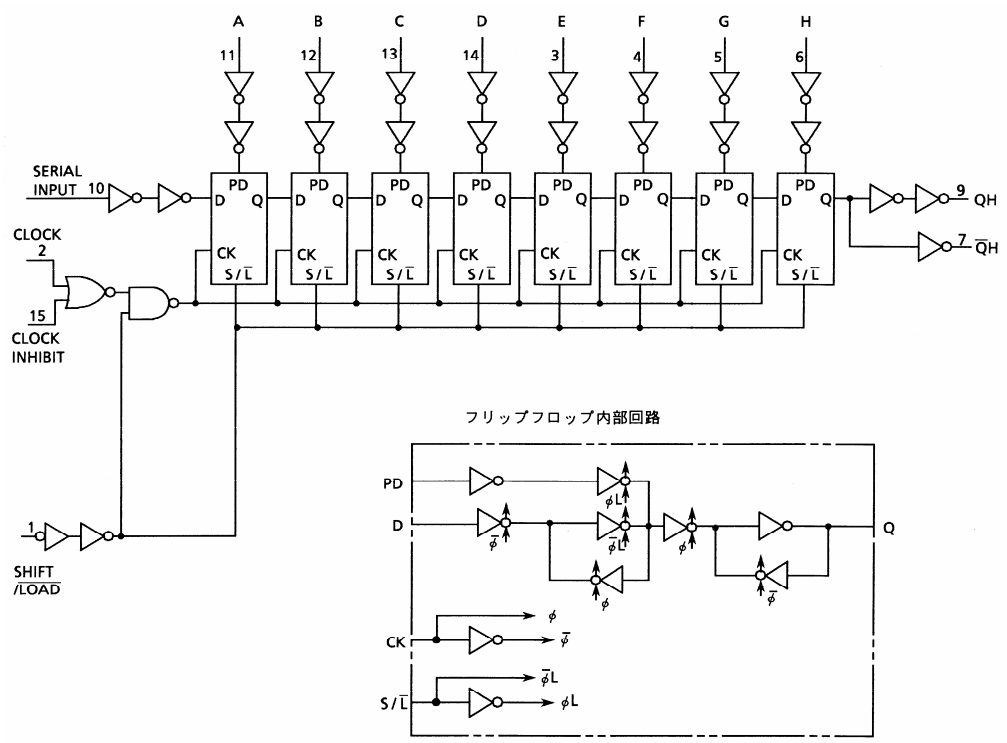
\includegraphics[width=0.8\linewidth]{figure/74165.png} 
    \caption{74ls165の内部回路} 
    \label{fig:74165}
\end{figure}

\begin{figure}[H]
    \centering
    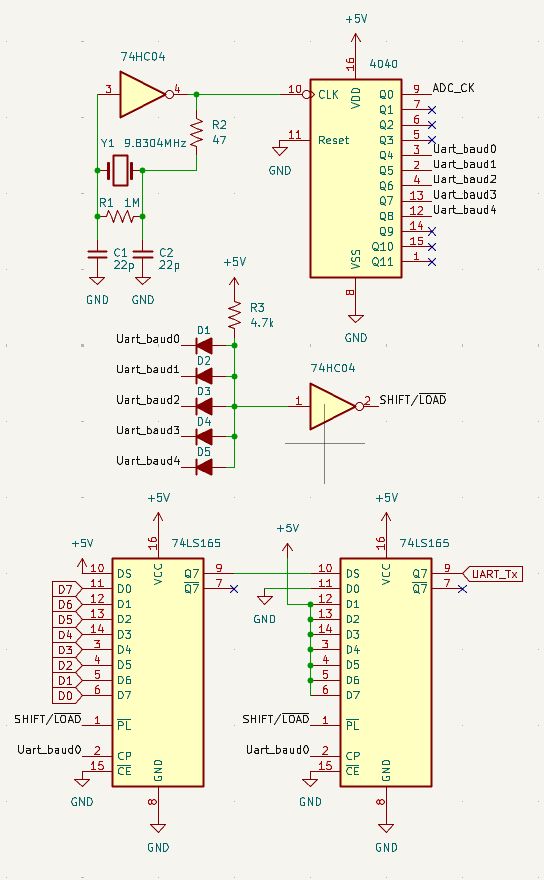
\includegraphics[width=\linewidth]{figure/uart_tx.png} 
    \caption{UART出力回路} 
    \label{fig:uart_tx}
\end{figure}

\subsubsection{LEDの駆動}
LED駆動回路は, 図\ref{fig:led}に示すように設計した.  
本研究で使用したLEDは, 浜松ホトニクス製のL12170である.  
このデバイスは外観こそ一般的な5mm LEDと同等のサイズであるが, 最大300\,mAという大電流を駆動できるうえ, 40\,MHzもの高速応答性を持っているという特徴がある.  

このLEDをフルパワーで駆動するには, ロジックICの出力能力では不十分である.  
そこで本設計ではMOSFETを用いた駆動回路を採用した.  
使用したMOSFETは$2SK4017$であり, このMOSFETのゲート容量はおよそ730\,pFある.
そのため,ロジックICの出力だけでは307.2\,kHzという比較的高い周波数でのスイッチングを安定して行うことができない.  

この問題に対応するため, ロジックICとMOSFETのゲートの間に, $2SC1815$と$2SA1015$を用いたプッシュプル回路を挿入している.  
これにより, MOSFETゲートの充放電が効率的に行われ, 高速スイッチング動作を安定させることができる.  
もちろん, 専用のゲートドライバICを用いればより理想的な駆動が実現できると考えられるが, 本回路では汎用トランジスタを組み合わせた簡易的な手法を採用している.

\begin{figure}[H]
    \centering
    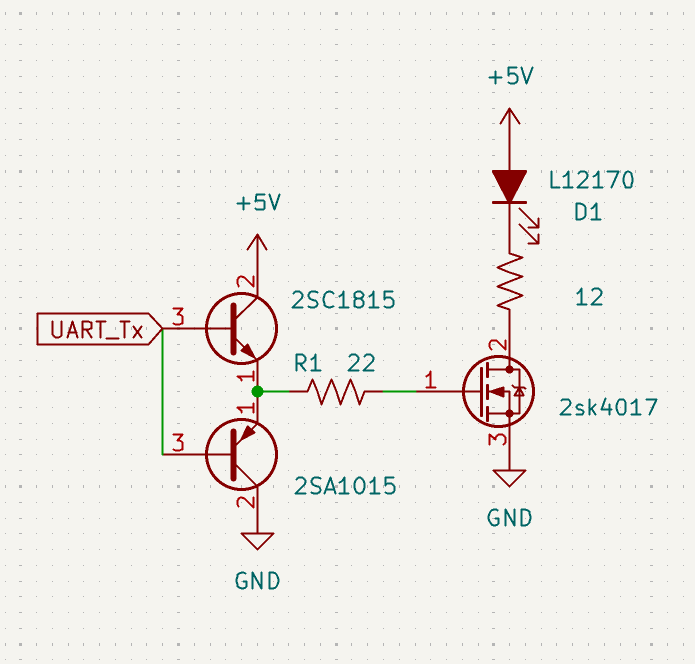
\includegraphics[width=\linewidth]{figure/led.png} 
    \caption{LED駆動回路} 
    \label{fig:led}
\end{figure}

\subsubsection{受光部分}
受光部分は図\ref{fig:tia}のように設計した.
この回路は受光素子に流れる微小な逆電流をロジックレベルの電圧に変換する.

受光素子は浜松ホトニクスのS6775である.
これは25MHzの高速応答,大きい受光面積による高い受光感度が特徴で,見た目がかっこいいので図\ref{fig:s6775}に示す.
使用したOPアンプはテキサスインスツルメンツのOPA350で,これは5V単電源でレールtoレールの出力,38MHzの広い利得帯域が特徴である.
これは今回扱う高速な微小電流を電圧に変換する回路に適している.
ひとつ1100円する.

この回路は前段と後段の2つのアンプで機能が分かれる.
前段はTIA本体で,後段はコンパレータである.
TIAの出力は2.5Vを中心に,受光素子から流れる電流によって±数十mVで振れる.
前段にある抵抗を大きくするとtiaがより大きい振幅の電圧を出力するようになる.
受光素子から流れる微小な電流をどこまで大きな電圧に変換できるかが通信距離を伸ばす上で要となる.
後段のコンパレータは2.5Vを中心に数mVのヒステリシスを持っており,TIAから電流が流れたかどうかを見てHigh,Lowを出力する.
TIA,コンパレータ,ともに逆相アンプで,二重にかけることで正相のアンプとして機能している.

この仕組みには疑問がある.
たとえば,光があたったときはダイオードから電流が流れる.
このとき,出力電圧が2.5 Vから2.4 Vになるとする.
それに対して光が当たっていないときは電流が流れないだけなので,出力電圧は2.5Vから変化しない.
このとき,コンパレータはこの回路のとおりに作るとしきい値が2.51Vぐらいになってしまって,これを上回れる場合は存在しなくなってしまう.
これは決着がついていないので,回路の基準電圧を作る部分を可変にして,その場で対応できるようにする.

\begin{figure}[H]
    \centering
    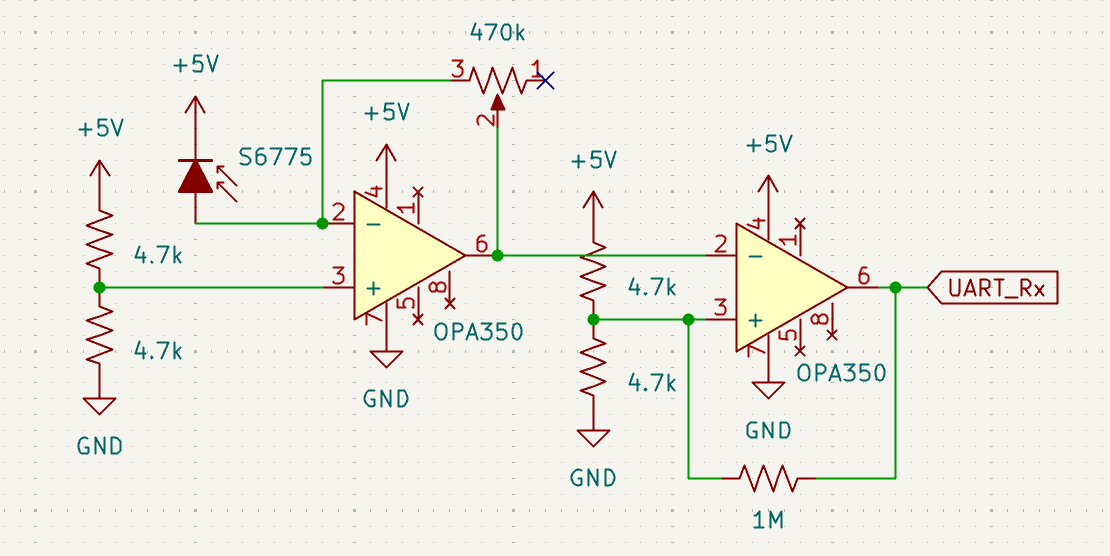
\includegraphics[width=1.4\linewidth,angle=270]{figure/tia.png} 
    \caption{入力側のアンプの回路} 
    \label{fig:tia}
\end{figure}

\begin{figure}[H]
    \centering
    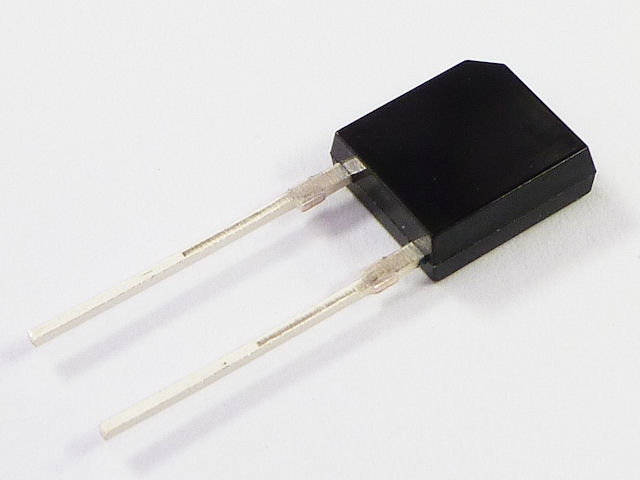
\includegraphics[width=\linewidth]{figure/s6775.jpg} 
    \caption{受光素子,S6775} 
    \label{fig:s6775}
\end{figure}
\newpage
\subsubsection{UARTの受信}
UART受信回路は図\ref{fig:uart_rx}のように設計した.
主な機能には74ls595を使用した.

74LS595の内部回路を図\ref{fig:74595}に示す.
これは8bitのシフトレジスタで,シリアルの信号をパラレルにして出力する.
74ls74はUARTの信号がLowになるタイミングを監視していて,Lowのエッジで$4040$の動作を可能にする.
$4040$はカウンタで,これが受信開始のタイミングで0からボーレートの立ち上がりまでクロックを数えると,UARTの信号とボーレートの信号の立ち上がりは1/2周期ずれることになる.
これが嬉しくて,ボーレートの立ち上がりのタイミングではUARTのデータはもっとも確からしい値を示している.
そのタイミングでシフトレジスタに取り込めば,UARTが受信できる.
これを9回繰り返せば,スタートbit+データbitを取り込んで,シフトレジスタにはちょうどデータだけが残り,受信が完了できる.
ダイオードロジックはそのタイミングを監視していて,受信が完了したらカウンタを止めることで受信を終わらせる.

\subsubsection{DAコンバータ}
UART受信回路は図\ref{fig:dac}のように設計した.
使用したICは$\mu PD6902$である.
これは映像信号用のDAコンバータで,$\mu PD6950$とは対になる存在らしい.
若松通商で800円で,在庫残り2だった.
出力についている$MCP602$はDACの出力を増強するものである.
貴重なICを壊したくないので,大事をとって入れてある.

$DAC\_CK$は行儀の悪い回路である.
図\ref{fig:uart_rx}を見ればわかるように,この信号はUARTの信号次第でいくらでもストレッチされる.
しかも,クロックが回るのは次のデータを受信している最中であるので,タイミング的にもなんだかややこい.

\begin{figure}[H]
    \centering
    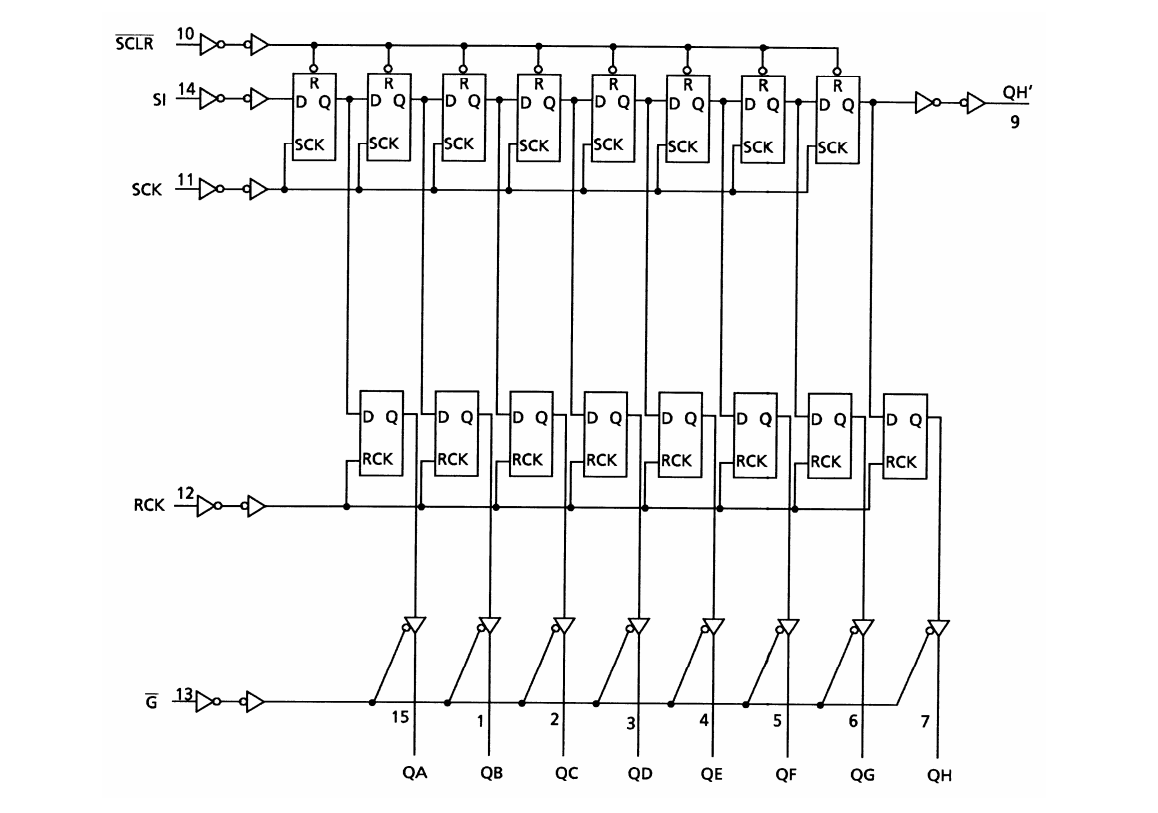
\includegraphics[width=\linewidth]{figure/74595.png} 
    \caption{74ls595の内部回路} 
    \label{fig:74595}
\end{figure}

\begin{figure}[H]
    \centering
    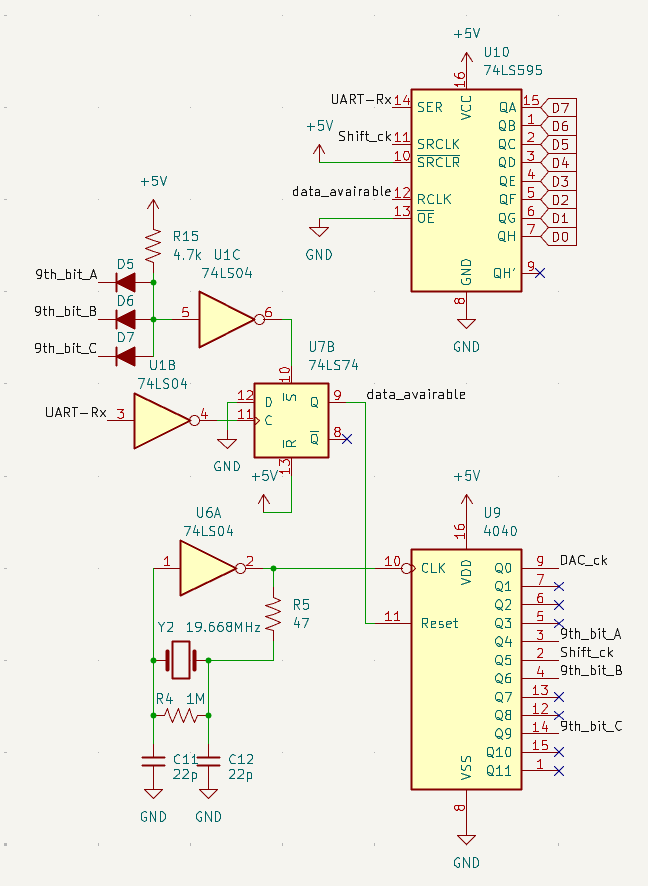
\includegraphics[width=\linewidth]{figure/uart_rx.png} 
    \caption{UART受信回路} 
    \label{fig:uart_rx}
\end{figure}

\begin{figure}[H]
    \centering
    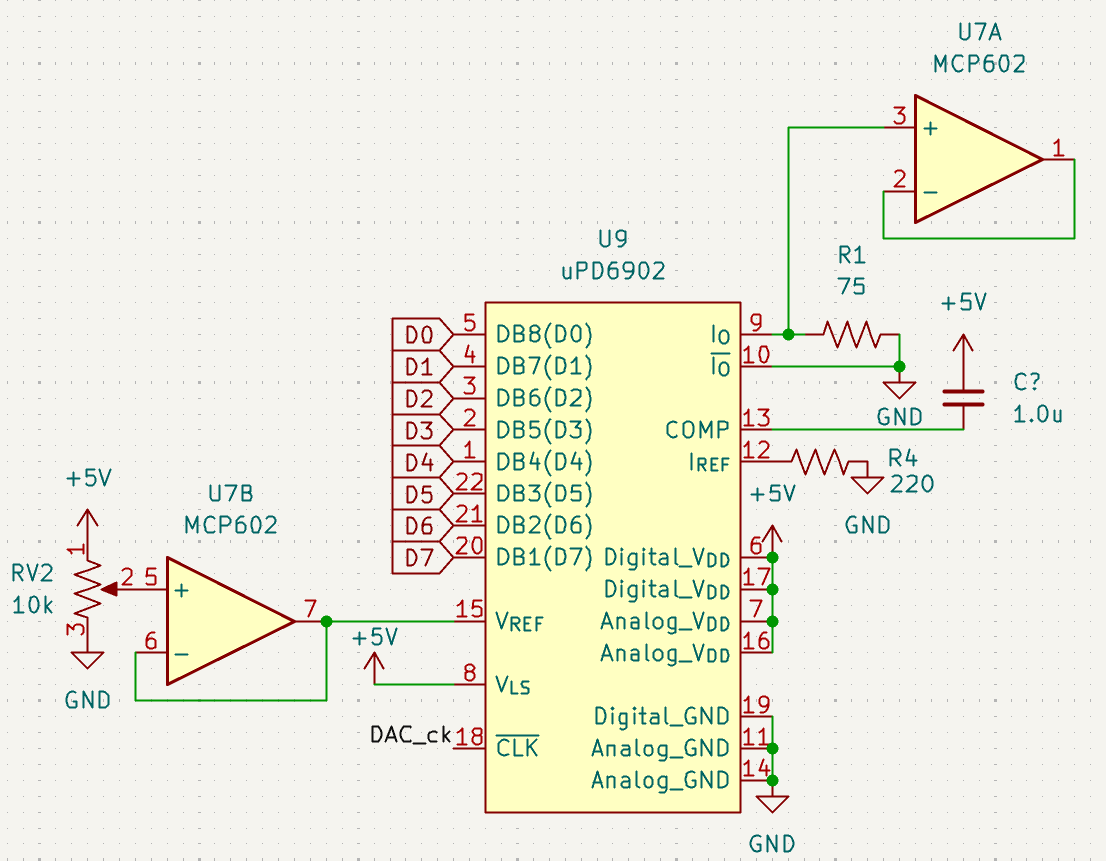
\includegraphics[width=\linewidth]{figure/dac.png} 
    \caption{DAコンバータ} 
    \label{fig:dac}
\end{figure}

\newpage
\subsubsection{出力側アンプ}
出力側アンプは図\ref{fig:out_amp}のように設計した.
使用したICはLM386で,回路はデータシートに記載のものをそのまま使用している.

\begin{figure}[H]
    \centering
    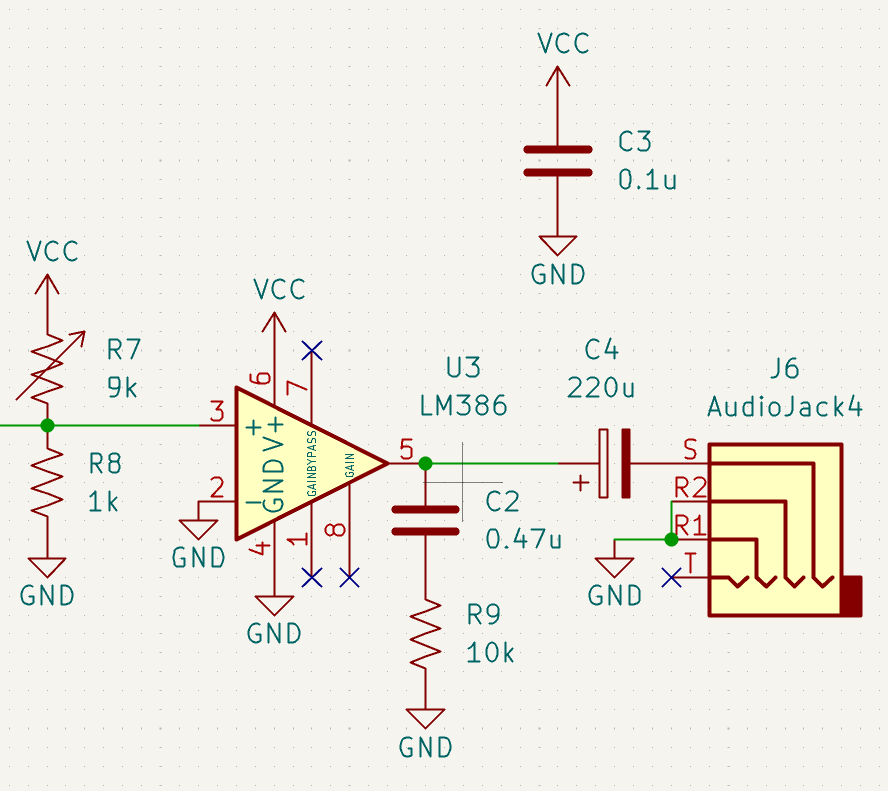
\includegraphics[width=\linewidth]{figure/out_amp.png} 
    \caption{出力側アンプ} 
    \label{fig:out_amp}
\end{figure}

\subsection{基板への実装}
基板に実装したものを図\ref{fig:sosin},\ref{fig:jusin}に示す.

\begin{figure}[H]
    \centering
    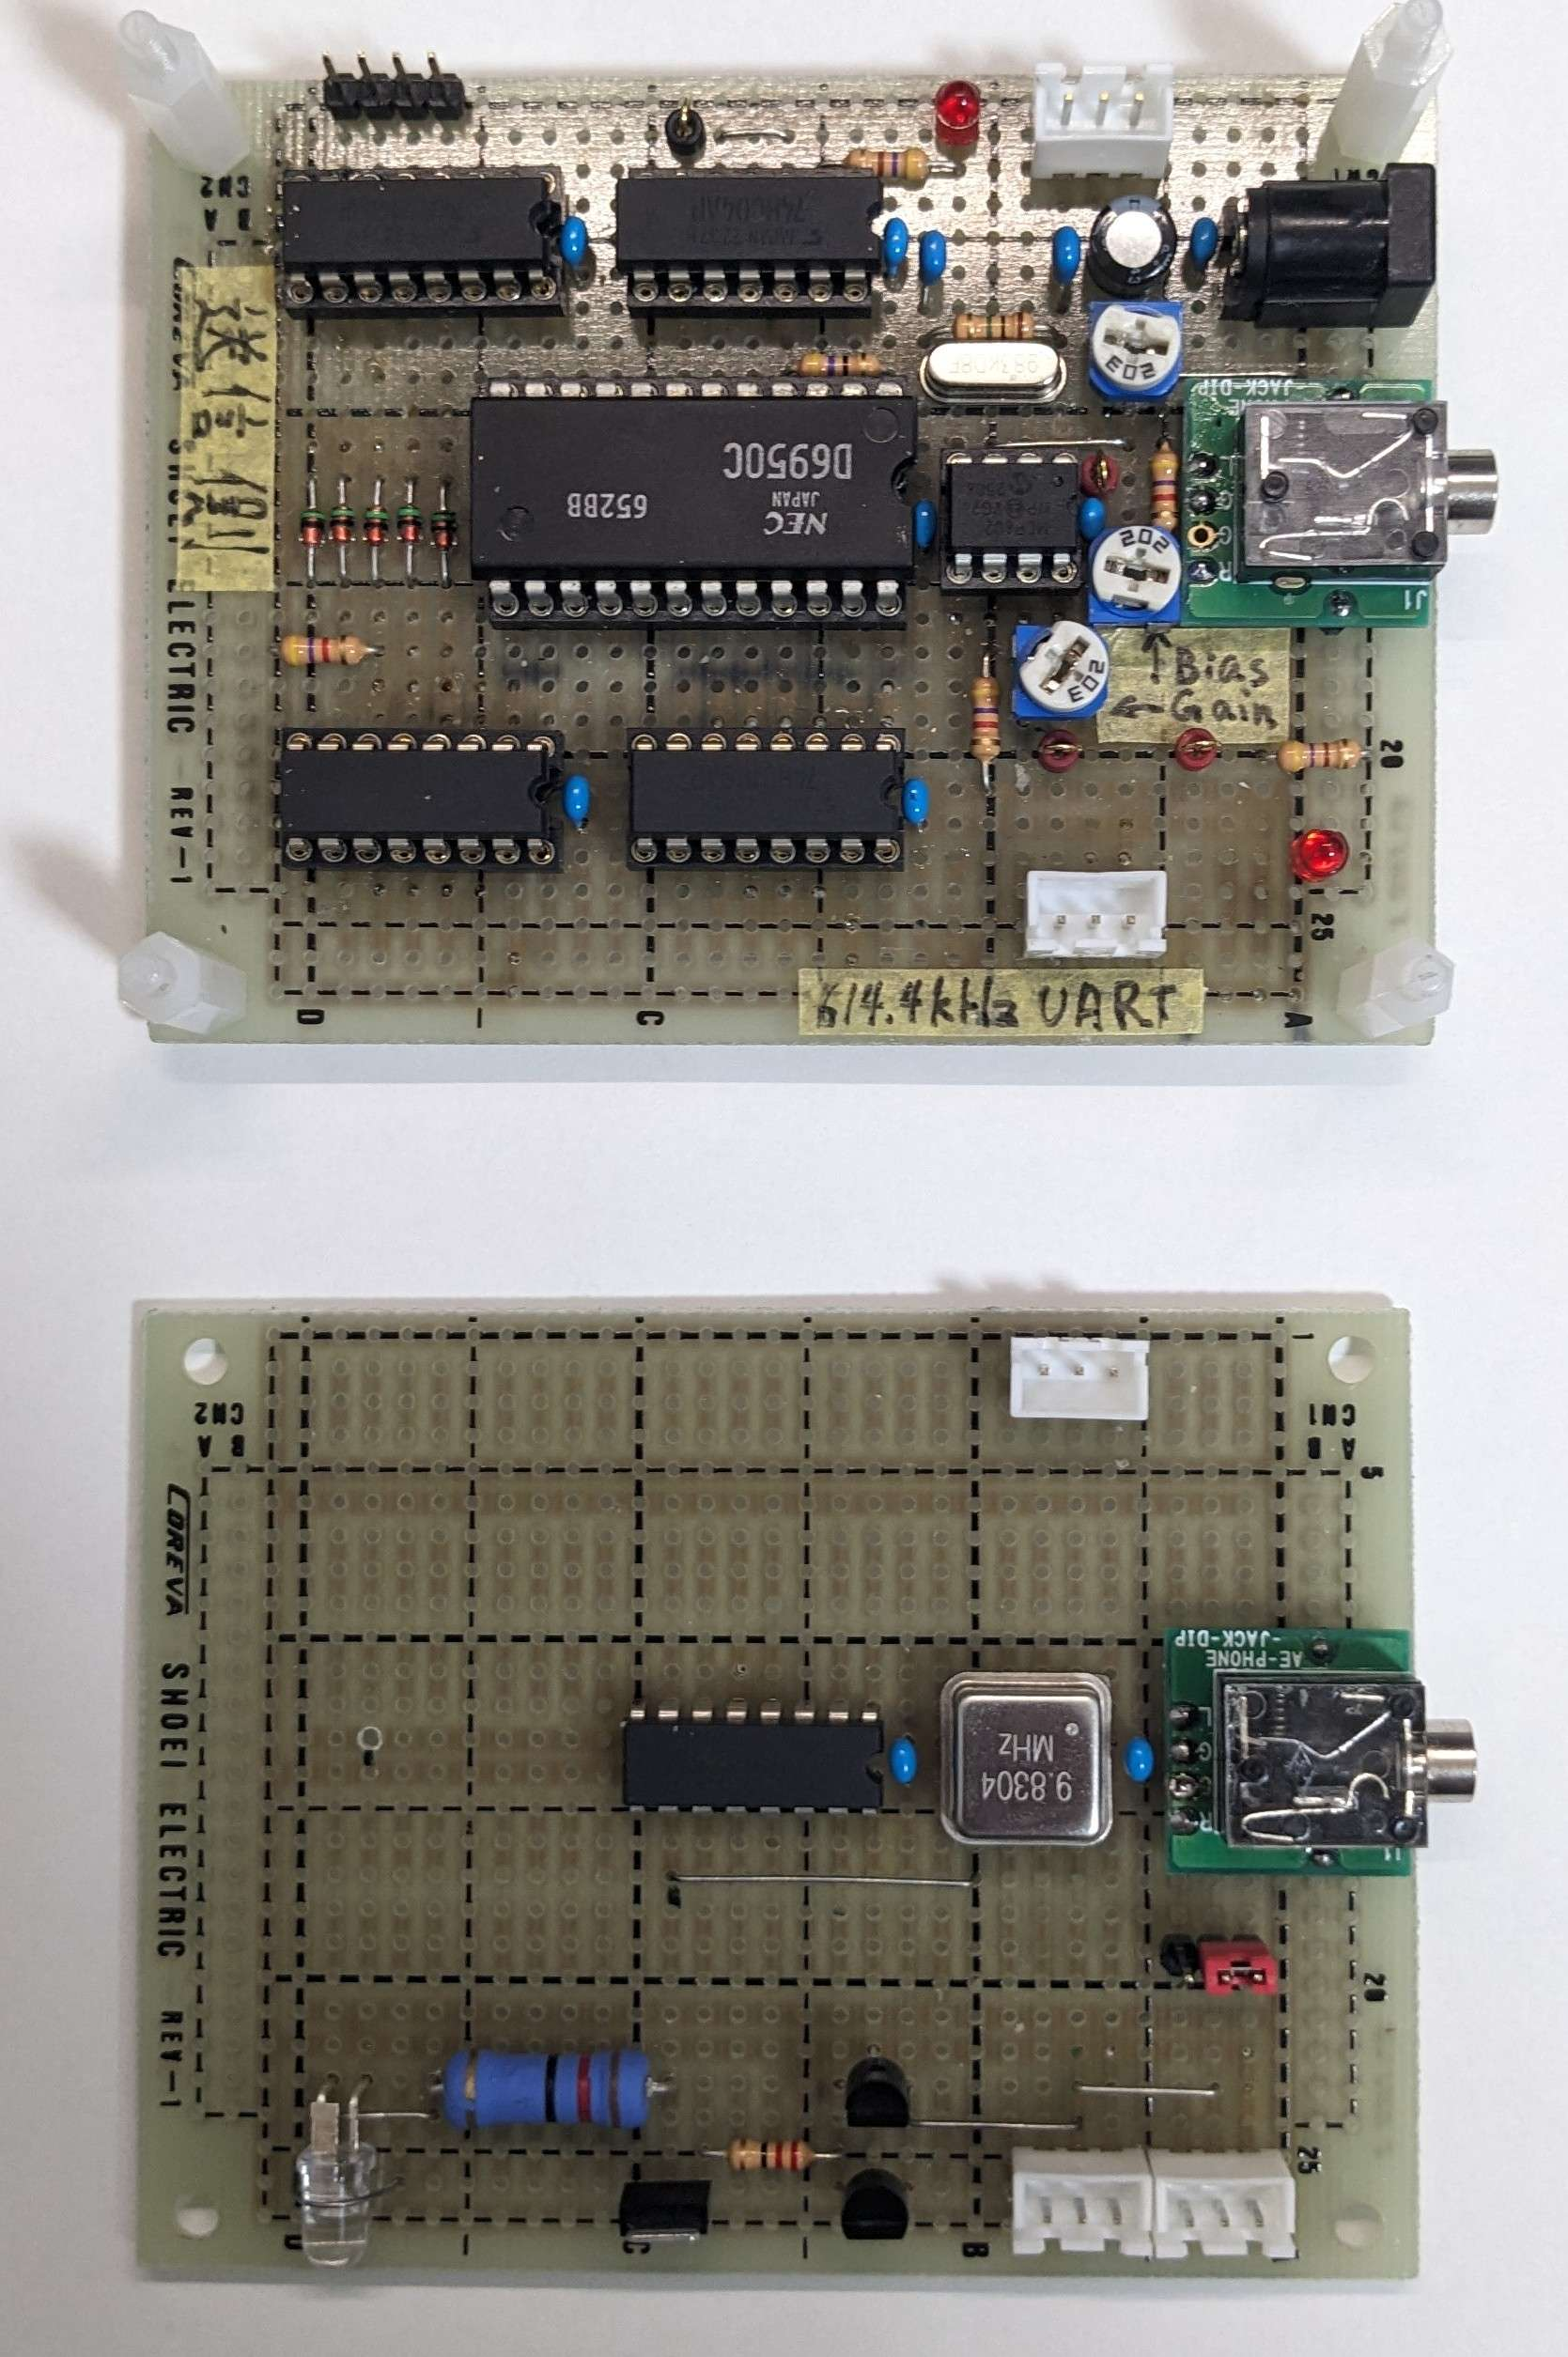
\includegraphics[width=0.8\linewidth]{figure/sosin.jpg} 
    \caption{送信側回路} 
    \label{fig:sosin}
\end{figure}

\begin{figure}[H]
    \centering
    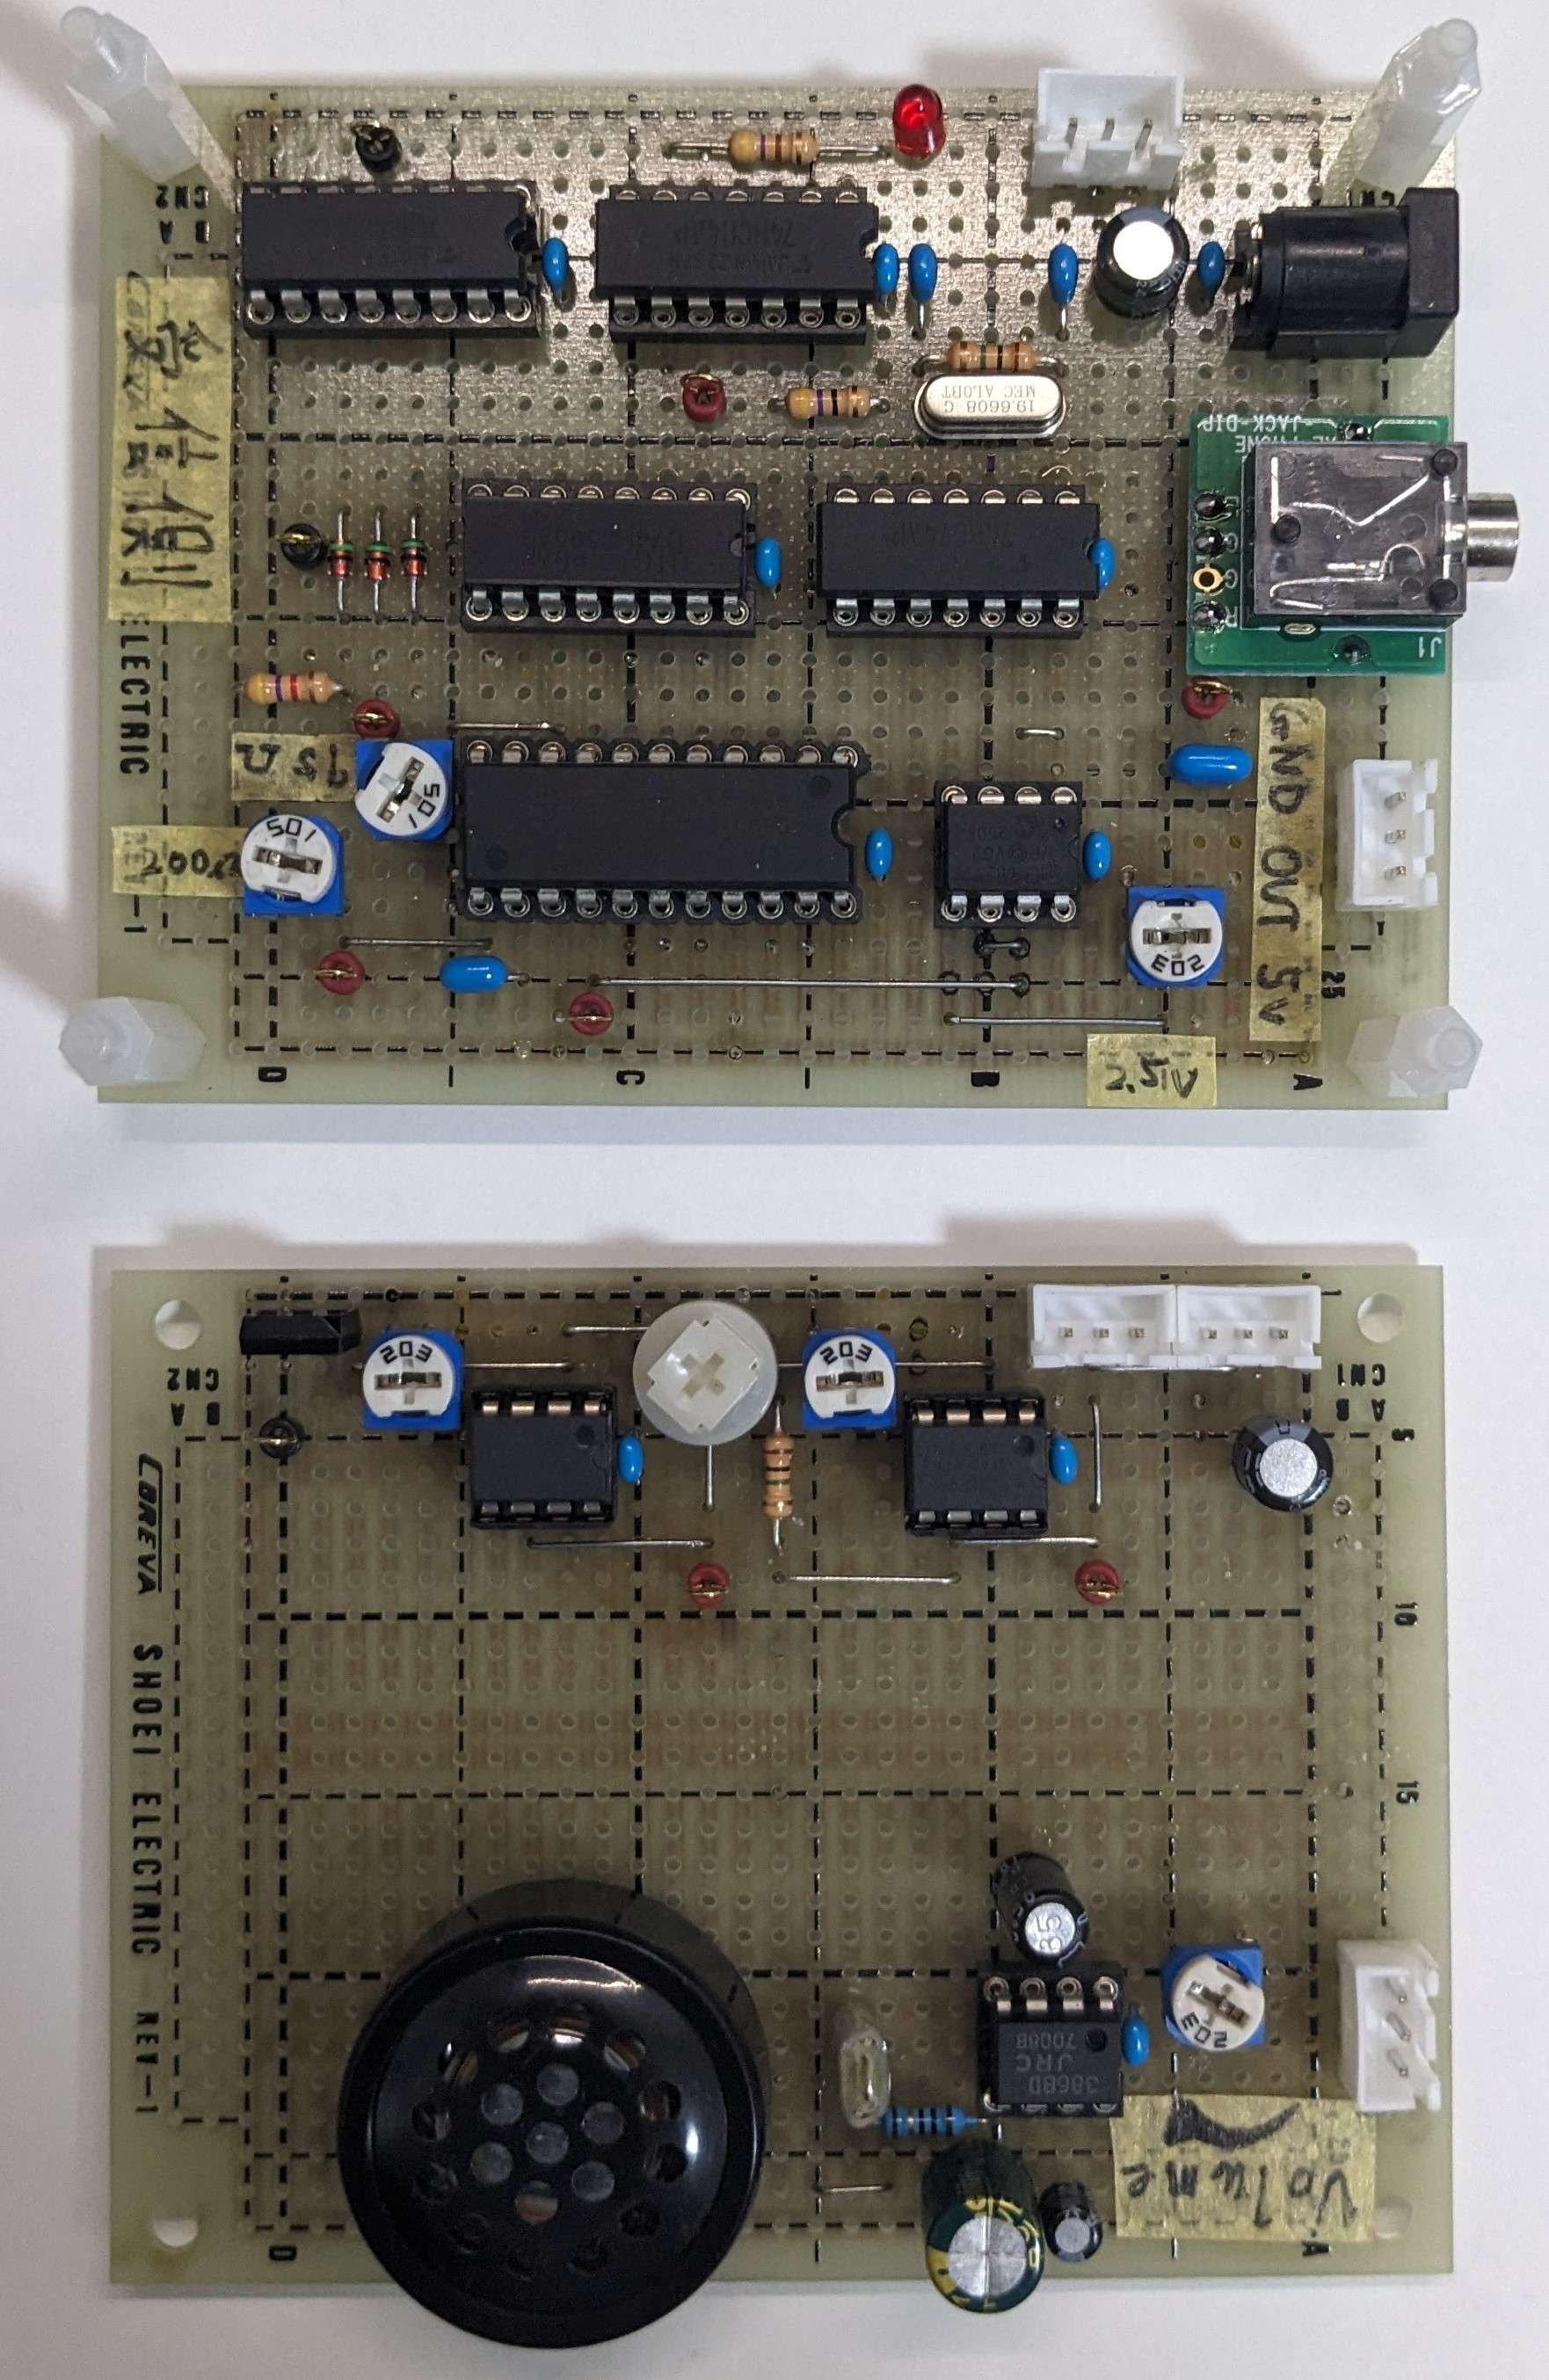
\includegraphics[width=0.8\linewidth]{figure/jusin.jpg} 
    \caption{受信側回路} 
    \label{fig:jusin}
\end{figure}
\subsection{動作確認}
図\ref{fig:test}, \ref{fig:check}に示すように, 通信が正常に行われていることを確認した.  
図\ref{fig:test}からは, 送信側で出力された波形が受信側で忠実に再現されていることがわかる.  
また, 図\ref{fig:check}では, PCのイヤホンジャックからの音声を受信側のスピーカで出力している様子を示している.  

\begin{figure}[H]
    \centering
    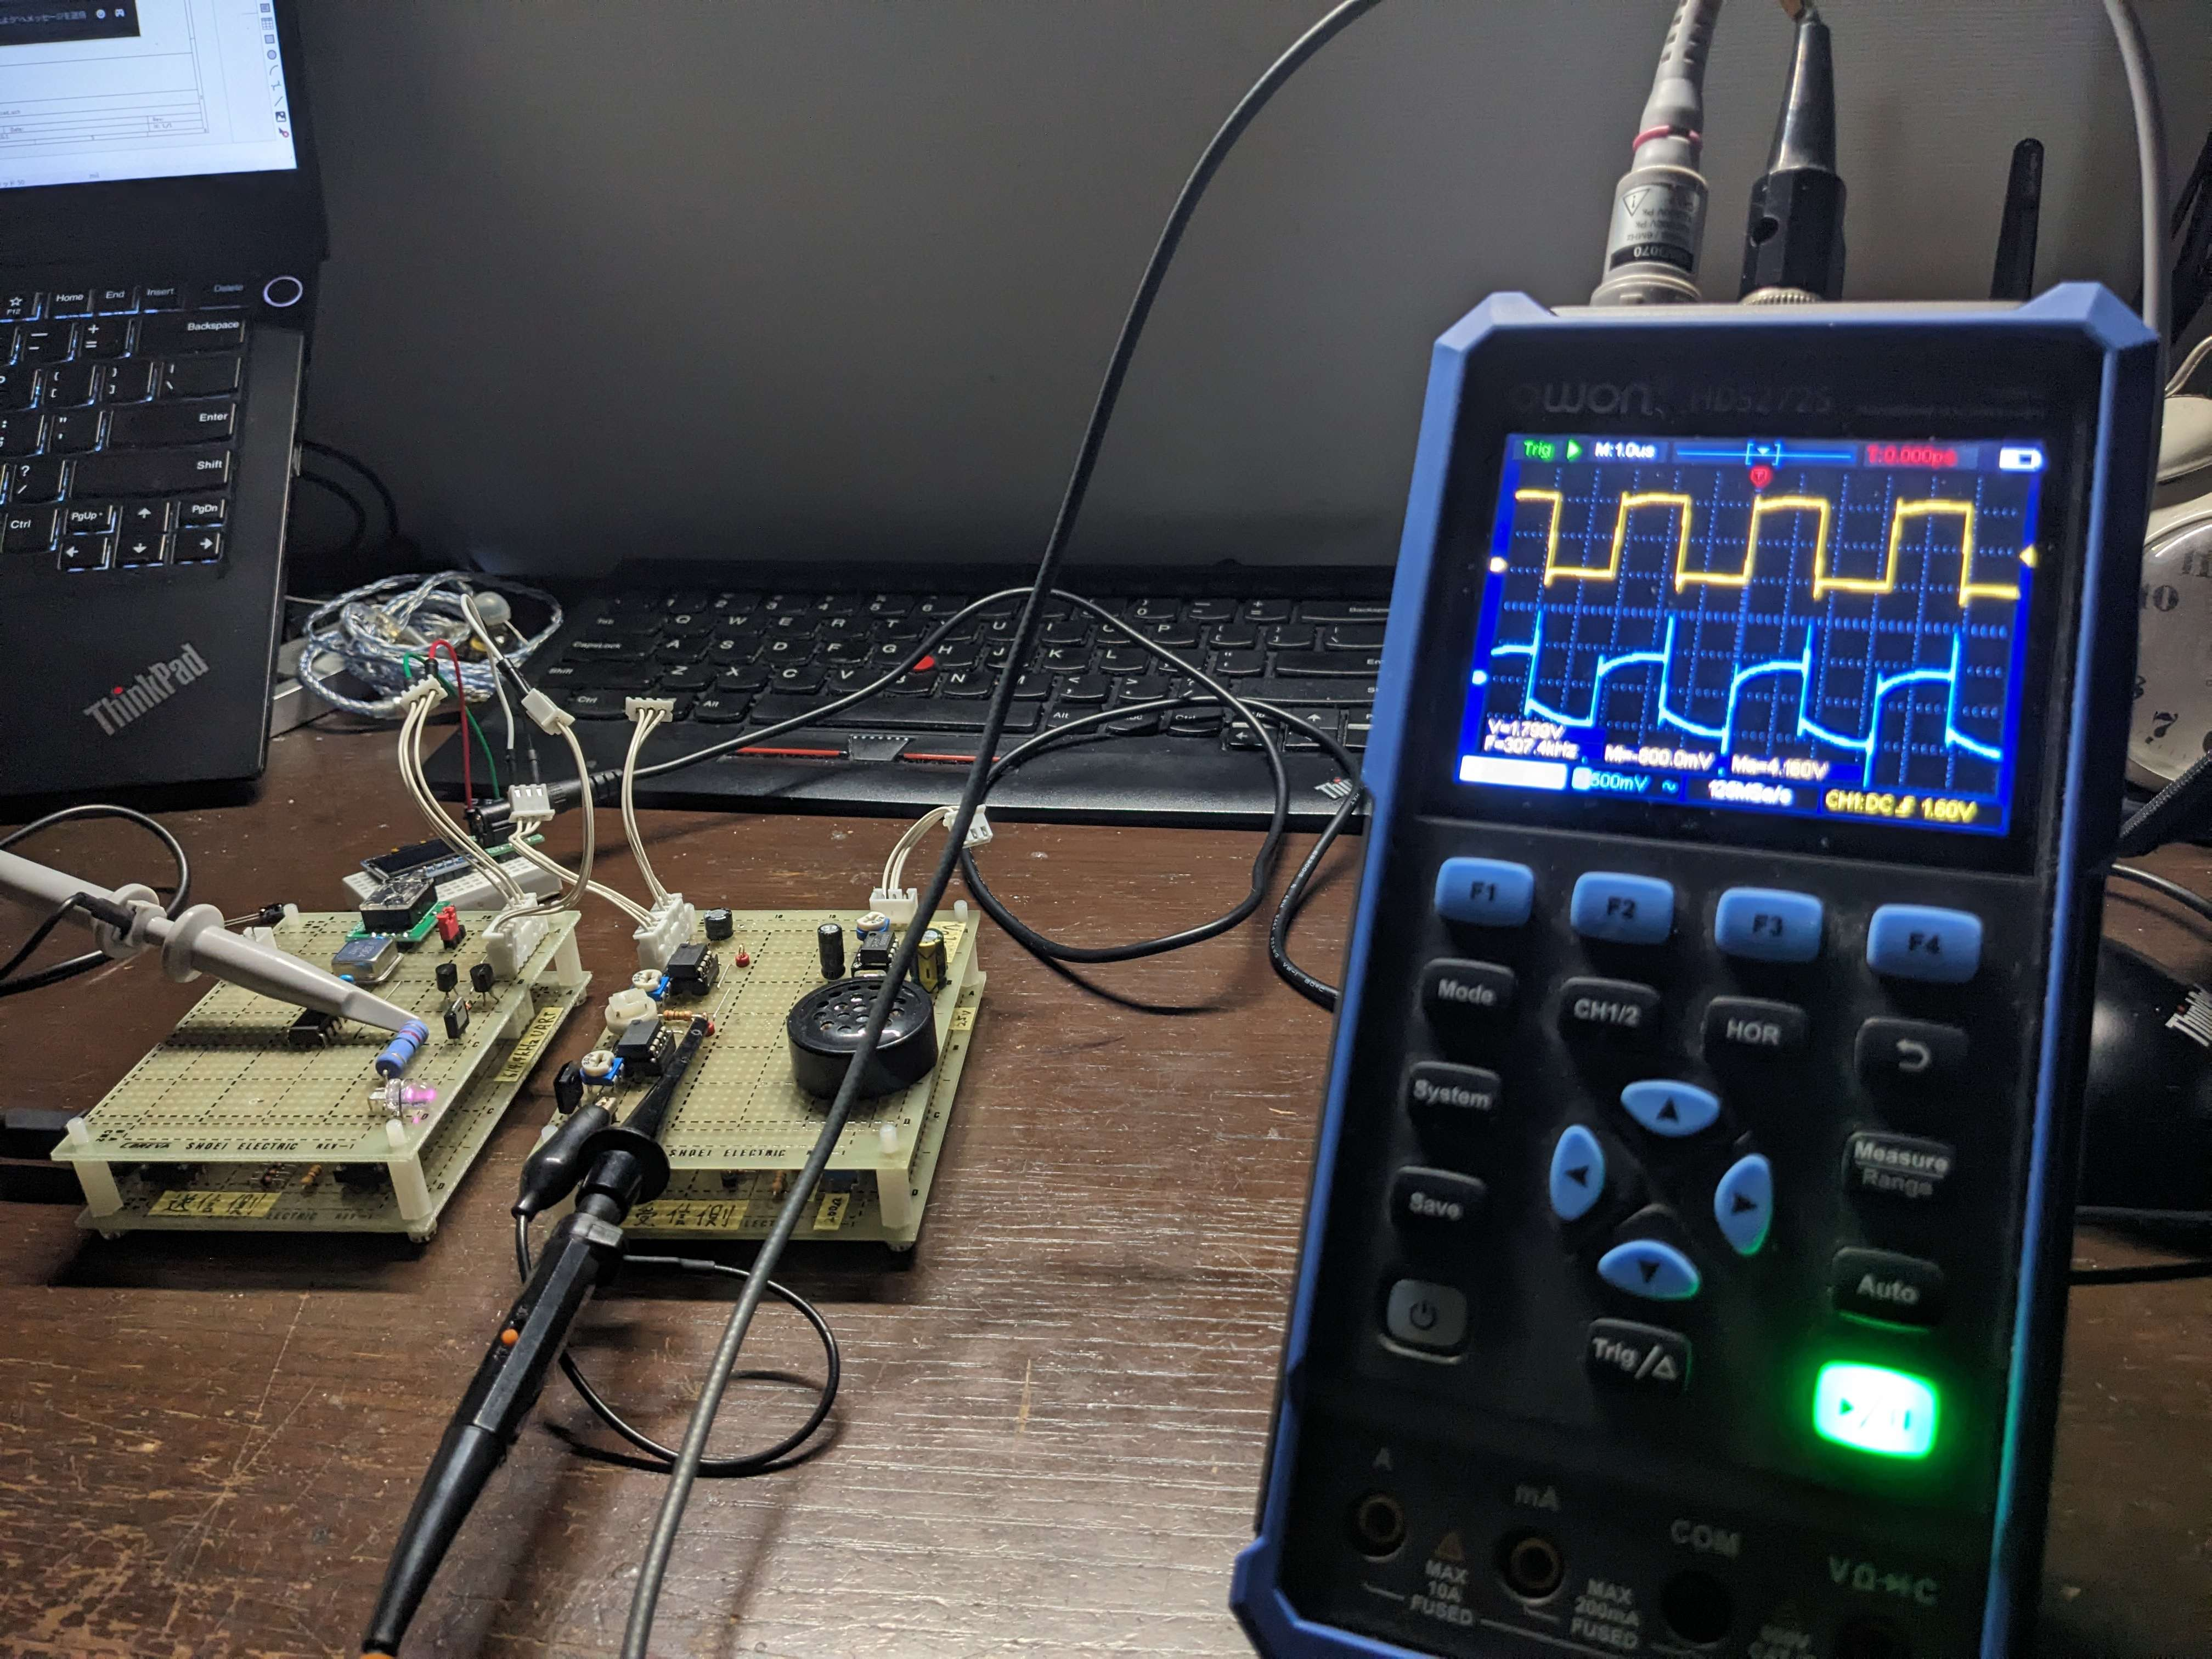
\includegraphics[width=0.7\linewidth]{figure/test.jpg} 
    \caption{通信の確認} 
    \label{fig:test}
\end{figure}

\begin{figure}[H]
    \centering
    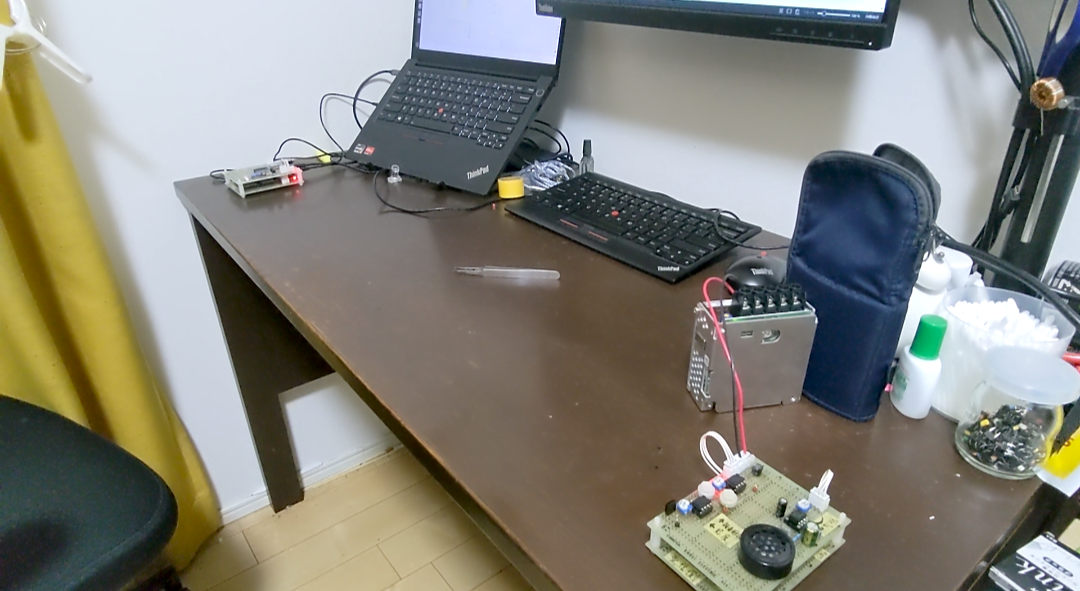
\includegraphics[width=0.7\linewidth]{figure/check.png} 
    \caption{動作確認} 
    \label{fig:check}
\end{figure}

この回路の通信距離は最大で約5\,mであった.
分解能は8bitしか無いが,サンプリング周波数がそれなり(19.2kHz)あるので,音質は十分であった(電話のサンプリング周波数は8kHz).
本来のノルマが1\,mなのでここで投げ出しても良いのだが,距離を追求してみることにする.

5\,m以上の距離では, 受光素子からの電流が不足し, TIAによって十分な振幅の電圧を得ることができなかった.  
この問題に対して, 以下のような解決策が考えられる.
\begin{itemize}
\item
  \textbf{LEDの高出力化}\\
  現在は1\,WクラスのLEDを1個のみ使用している.  
  これを2個, 8個, 32個と増設すれば, 受光素子に流れる電流も増加すると考えられる.  
  ただし, LEDは1個あたり約300円と高価であり, コスト面が課題となる.  

\item
  \textbf{受光素子の増設}\\
  受光素子を並列に追加することで, 電流を単純に増加させることができると期待される.  
  しかし, 受光素子は数百\,nAオーダーの微弱な電流しか流れず非常にデリケートであるため, この方法の有効性には不確実性がある.
  少なくとも,そのような前例は見つけられなかった.

\item
  \textbf{パラボラアンテナの利用}\\
  大きな面積で集光し, 受光素子に光を集中させることで, LEDや受光素子を改造せずとも通信距離の延長が可能となる.  
  ただし, 大型の装置を製作する必要がある点が課題である.  
\end{itemize}

実際に林がパラボラアンテナを試作し, これを用いてテストを行ったところ, 通信距離は約10\,mまで延長できた.  
今後はこのアプローチを基盤として, 通信距離のさらなる改善を図ることとする.

\section{今後の予定}
パラボラアンテナをつくって,通信距離を伸ばす.

\section{稲毛研に勝てるか}
勝てる.


\vfill
\end{multicols}

\end{document}
